\clearpage
\begingroup
\let\clearpage\relax
\let\cleardoublepage\relax
\vspace*{\fill}
\chapter{项目管理与质量}
\begin{center}
项目管理回答四个问题：\textbf{要多久、花多少、有多少风险、质量如何度量}。本章沿「估算--进度--风险--质量」四步展开，把成本模型、关键路径法、风险应对与质量度量落到可计算的公式与表格上。
\end{center}
\vspace*{\fill}
\endgroup
\clearpage

\section{规模与成本估算}

\subsection{代码行 LOC 与功能点 FP}

\textbf{代码行 (LOC, Lines of Code)} 是最直观的规模度量，通常以千行 \textbf{KLOC} 为单位。它易于统计，但依赖语言与编程风格，且在设计完成前难以准确预估。

\textbf{功能点 (FP, Function Points)} 从「用户可见的功能」出发，与语言无关。先按复杂度给五类功能元素加权，得到未调整功能点 $UFP$：

\begin{table}[H]
\centering
\caption{功能点五类元素及复杂度权重}
\begin{tabulary}{\textwidth}{LCCC}
\toprule
功能元素 & 简单 & 平均 & 复杂 \\
\midrule
外部输入 EI & 3 & 4 & 6 \\
外部输出 EO & 4 & 5 & 7 \\
外部查询 EQ & 3 & 4 & 6 \\
内部逻辑文件 ILF & 7 & 10 & 15 \\
外部接口文件 EIF & 5 & 7 & 10 \\
\bottomrule
\end{tabulary}
\end{table}

再用 14 项通用系统特征（数据通信、性能、重用性等）的复杂度 $F_i\in[0,5]$ 做调整：

\begin{equation}
    FP = UFP \times \left(0.65 + 0.01\sum_{i=1}^{14} F_i\right)
\end{equation}

其中调整因子取值范围为 $0.65\sim1.35$。功能点可在设计前估算，再换算成 KLOC 以套用成本模型。

\subsection{COCOMO 模型}

\textbf{COCOMO (Constructive Cost Model)} 把工作量表示为规模的幂函数。基本模型按项目类型取参数 $a,b,c,d$：

\begin{table}[H]
\centering
\caption{COCOMO 基本模型参数}
\begin{tabulary}{\textwidth}{LCCC}
\toprule
项目类型 & $a$ & $b$ & 说明 \\
\midrule
组织型 (Organic) & 2.4 & 1.05 & 小型、经验丰富、约束少 \\
半独立型 (Semi-detached) & 3.0 & 1.12 & 中等规模、混合经验 \\
嵌入式 (Embedded) & 3.6 & 1.20 & 硬约束、复杂接口 \\
\bottomrule
\end{tabulary}
\end{table}

\noindent 组织型对应的基本公式为

\begin{equation}
    E = 2.4 \times (KLOC)^{1.05} \quad \text{(人月, person-months)}
\end{equation}
\begin{equation}
    D = 2.5 \times E^{0.38} \quad \text{(开发月数, months)}
\end{equation}
\begin{equation}
    \text{团队规模} = \frac{E}{D} \quad \text{(人)}
\end{equation}

\noindent 例如 $KLOC=33$（组织型）时：$E=2.4\times33^{1.05}\approx94.3$ 人月，$D=2.5\times94.3^{0.38}\approx14.1$ 月，团队规模约 $6.7$ 人。可见工作量随规模\textbf{超线性}增长——把规模翻倍，工作量增长超过一倍，这正是「人月神话」的量化根源。

\begin{table}[H]
\centering
\caption{常用成本估算方法对比}
\begin{tabulary}{\textwidth}{LLL}
\toprule
方法 & 优点 & 局限 \\
\midrule
代码行 LOC & 直观、易统计 & 语言相关、需设计后 \\
功能点 FP & 与语言无关、早期可用 & 主观、需经验校准 \\
COCOMO & 公式化、可调参 & 依赖历史数据与规模估计 \\
\bottomrule
\end{tabulary}
\end{table}

\section{进度计划}

\subsection{甘特图}

\textbf{甘特图 (Gantt Chart)} 用横条表示各活动的起止时间，直观展示进度与并行关系，是沟通与跟踪的主力工具。下面是本章示例项目的甘特图（时间单位统一，关键活动以深色标出）：

\begin{figure}[H]
\centering
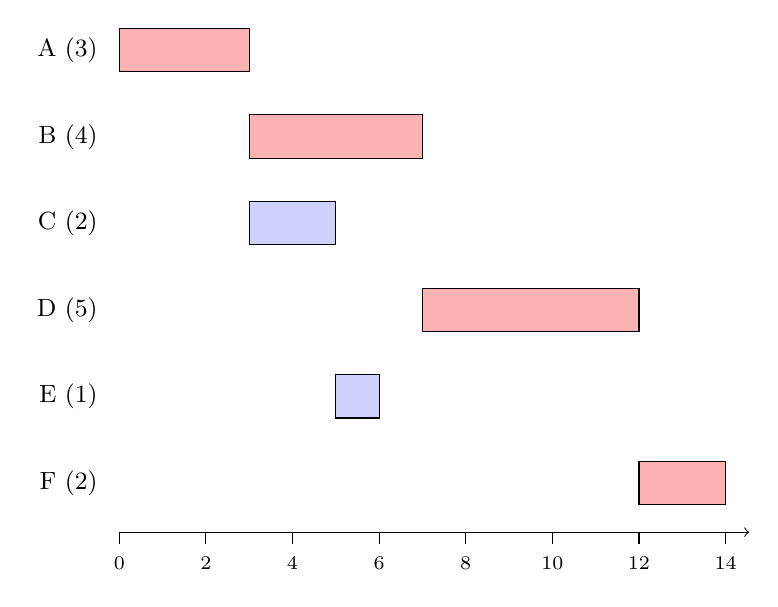
\begin{tikzpicture}[font=\small]
    \def\s{0.55}
    % ---- 活动行 ----
    \node[anchor=east] at (-0.15,5.27) {A (3)};
    \draw[fill=red!30] (0,5.0) rectangle ({3*\s},5.55);
    \node[anchor=east] at (-0.15,4.17) {B (4)};
    \draw[fill=red!30] ({3*\s},3.9) rectangle ({7*\s},4.45);
    \node[anchor=east] at (-0.15,3.07) {C (2)};
    \draw[fill=blue!18] ({3*\s},2.8) rectangle ({5*\s},3.35);
    \node[anchor=east] at (-0.15,1.97) {D (5)};
    \draw[fill=red!30] ({7*\s},1.7) rectangle ({12*\s},2.25);
    \node[anchor=east] at (-0.15,0.87) {E (1)};
    \draw[fill=blue!18] ({5*\s},0.6) rectangle ({6*\s},1.15);
    \node[anchor=east] at (-0.15,-0.23) {F (2)};
    \draw[fill=red!30] ({12*\s},-0.5) rectangle ({14*\s},0.05);
    % ---- 时间轴 ----
    \draw[->] (0,-0.85) -- ({14*\s+0.3},-0.85);
    \foreach \x in {0,2,4,6,8,10,12,14} {
        \draw (\x*\s,-0.85) -- (\x*\s,-1.0);
        \node[font=\scriptsize] at (\x*\s,-1.25) {\x};
    }
\end{tikzpicture}
\caption{项目甘特图（深色为关键活动，括号内为工期）}
\end{figure}

\subsection{PERT 与关键路径法 CPM}

\textbf{关键路径法 (CPM)} 把项目建成\textbf{活动在网络 (AON)}：节点是活动，箭头表示先后约束。对每个活动计算四个时间：

\begin{itemize}
    \item 最早开始 $ES$、最早完成 $EF = ES + \text{工期}$：沿网络\textbf{正向}推进，$ES=\max(\text{所有前置的 } EF)$。
    \item 最晚完成 $LF$、最晚开始 $LS = LF - \text{工期}$：沿网络\textbf{反向}推进，$LF=\min(\text{所有后继的 } LS)$，终点 $LF$ 取项目总工期。
\end{itemize}

\textbf{总浮动时间 (Total Float)} 为

\begin{equation}
    TF = LS - ES = LF - EF
\end{equation}

$TF=0$ 的活动组成\textbf{关键路径}，其长度等于项目最短工期；关键活动一旦延误，整个项目立即延误。示例项目活动与计算结果如下：

\begin{table}[H]
\centering
\caption{示例项目活动表与 CPM 计算结果}
\begin{tabulary}{\textwidth}{CCCCCCCC}
\toprule
活动 & 工期 & 前置 & $ES$ & $EF$ & $LS$ & $LF$ & $TF$ \\
\midrule
A & 3 & -- & 0 & 3 & 0 & 3 & 0 \\
B & 4 & A & 3 & 7 & 3 & 7 & 0 \\
C & 2 & A & 3 & 5 & 9 & 11 & 6 \\
D & 5 & B & 7 & 12 & 7 & 12 & 0 \\
E & 1 & C & 5 & 6 & 11 & 12 & 6 \\
F & 2 & D, E & 12 & 14 & 12 & 14 & 0 \\
\bottomrule
\end{tabulary}
\end{table}

\noindent 关键路径为 $A \to B \to D \to F$，工期 $3+4+5+2=14$。活动 C、E 各有 6 个时间单位的浮动，可在不影响总工期的前提下适当推迟或调配资源。

\section{风险管理}

\subsection{风险识别与评估}

\textbf{风险}是「尚未发生、但一旦发生会危害项目」的潜在事件。管理流程为：识别 $\to$ 分析（概率 $\times$ 影响）$\to$ 制定应对 $\to$ 监控。风险值用「发生概率」与「影响程度」的乘积度量：

\begin{equation}
    R = P(\text{风险}) \times I(\text{影响})
\end{equation}

\noindent 常见风险来源分四类：\textbf{技术}（技术不成熟、需求不稳）、\textbf{人员}（流失、技能不足）、\textbf{组织}（预算削减、变更失控）、\textbf{外部}（供应商、法规）。下表给出典型风险登记册：

\begin{table}[H]
\centering
\caption{风险登记册示例（概率、影响取 $1\sim5$）}
\begin{tabulary}{\textwidth}{LCCCL}
\toprule
风险 & 概率 $P$ & 影响 $I$ & $R=P\times I$ & 应对策略 \\
\midrule
需求蔓延 & 4 & 4 & 16 & 缓解：变更控制、原型确认 \\
关键技术不成熟 & 3 & 4 & 12 & 规避：技术预研、留备选 \\
核心人员流失 & 2 & 5 & 10 & 缓解：文档化、结对、备份 \\
第三方组件延误 & 3 & 3 & 9 & 转移：合同条款、多供应商 \\
预算削减 & 3 & 5 & 15 & 缓解/接受：优先级排序与储备 \\
\bottomrule
\end{tabulary}
\end{table}

\subsection{风险应对策略}

针对高 $R$ 值风险，需选择并落实应对策略：

\begin{itemize}
    \item \textbf{规避 (Avoid)}：改变计划以消除风险源，如采用成熟技术替代未验证方案。
    \item \textbf{转移 (Transfer)}：把后果转给第三方，如外包、保险、固定价合同。
    \item \textbf{缓解 (Mitigate)}：降低发生概率或影响，如增加评审、冗余设计、缓冲。
    \item \textbf{接受 (Accept)}：风险影响小或应对成本过高时，预留应急储备并监控。
\end{itemize}

\begin{table}[H]
\centering
\caption{概率--影响矩阵与处置建议}
\begin{tabulary}{\textwidth}{CCCC}
\toprule
 & 影响低 & 影响中 & 影响高 \\
\midrule
概率高 & 缓解 & 缓解/规避 & 规避/转移 \\
概率中 & 接受 & 缓解 & 规避/转移 \\
概率低 & 接受 & 接受 & 缓解/转移 \\
\bottomrule
\end{tabulary}
\end{table}

\noindent 风险管理的输出是可跟踪的\textbf{风险登记册}与\textbf{应急储备}：不仅登记风险，还要指定负责人、触发条件与应对动作，并随项目推进持续复审。

\section{软件质量}

\subsection{ISO 质量模型}

\textbf{ISO/IEC 9126}（后演化为 ISO/IEC 25010）从多个质量特性刻画软件质量，常归纳为「功能性、可靠性、易用性、效率、可维护性、可移植性」等：

\begin{table}[H]
\centering
\caption{ISO 质量特性}
\begin{tabulary}{\textwidth}{LL}
\toprule
质量特性 & 含义 \\
\midrule
功能性 (Functionality) & 满足所声明与隐含需求的能力 \\
可靠性 (Reliability) & 在规定条件下维持规定性能的能力 \\
易用性 (Usability) & 被理解、学习、使用的难易程度 \\
效率 (Efficiency) & 时间与资源利用的效率 \\
可维护性 (Maintainability) & 被修改、纠错、适应、完善的能力 \\
可移植性 (Portability) & 迁移到其他环境的能力 \\
\bottomrule
\end{tabulary}
\end{table}

\subsection{质量度量}

质量特性需用可度量的指标落地。常用度量包括：

\begin{equation}
    D = \frac{\text{缺陷总数}}{\text{KLOC}} \quad \text{(缺陷密度, defects/KLOC)}
\end{equation}
\begin{equation}
    MTBF = MTTF + MTTR
\end{equation}
\begin{equation}
    A = \frac{MTTF}{MTTF + MTTR} \quad \text{(可用度, Availability)}
\end{equation}

其中 $MTTF$ 为平均无故障时间，$MTTR$ 为平均修复时间。由公式可见：提高可用度有两条路——\textbf{降低故障率}（增大 $MTTF$）或\textbf{加快恢复}（减小 $MTTR$）。工程上常在两者间权衡，例如高可用系统用冗余提高 $MTTF$、用自动故障转移压缩 $MTTR$。

\begin{table}[H]
\centering
\caption{常用质量度量指标}
\begin{tabulary}{\textwidth}{LLL}
\toprule
指标 & 定义 & 关注点 \\
\midrule
缺陷密度 & 缺陷数 / KLOC & 开发与测试阶段的缺陷控制 \\
可靠性 & 失效概率、$MTTF$ & 长时间稳定运行能力 \\
$MTBF$ & $MTTF+MTTR$ & 平均故障间隔，可维护系统 \\
可用度 $A$ & $MTTF/MTBF$ & 服务可用的时间占比 \\
\bottomrule
\end{tabulary}
\end{table}

\noindent 度量本身不是目的：质量模型提供「看哪些维度」，度量提供「量多大」，而评审、测试与过程改进才是「把质量做出来」的手段。
